\usetikzlibrary{arrows, decorations.markings}
\usetikzlibrary{trees}

\tikzstyle{level 1}=[level distance=1cm, sibling distance=1.5cm]
\tikzstyle{level 2}=[level distance=1cm, sibling distance=1.1cm]

% Define styles for operators and leafs
\tikzstyle{operator} = [draw=none,circle, minimum width=1pt]
\tikzstyle{end} = [circle, minimum width=3pt,fill, inner sep=0pt]
% for double arrows a la chef
% adapt line thickness and line width, if needed

\begin{subfigure}[b]{0.49\textwidth}\centering
\begin{tikzpicture}[thick]

 \node[] (base_kernels) {\small$\text{BK}=\{k_{\bm{\theta}^1}^1,\cdots,k_{\bm{\theta}^m}^m\}$};
 \node[above=0.7cm of base_kernels] (theta) {\small$\bm{\theta}^* \sim P(\bm{\theta}^*)$};
 \node[draw,rectangle, below=1cm of start, text width =6.0cm, text 
height=4.1cm,align=center] (grammar)
{};


 \node[draw,dashed,rectangle, below=-3.8cm of grammar, text width
=5.3cm,align=center] (subset) {
$\;$Select Primitive Kernels\\% I can't believe that this is the simpliest way to
% get spacing right 
{\raggedright
\footnotesize$\Sbf  \sim P(\Sbf =
\{k_{\bm{\theta}^i}^i,\cdots,k_{\bm{\theta}^n}^n\} \mid \text{BK})$
}
};
 \node[draw,rectangle,dashed, below=0.7cm of subset, text width
=4.35cm,align=center]
(composition_procedure) {
$\;$Kernel Composer\\ % I can't believe that this is the simpliest way to
% get spacing right 
{\raggedright
\footnotesize$\;\;\;\bm{\Omega} \sim P(\bm{\Omega} \mid \Sbf)$ \\

\footnotesize$k_{\bm{\theta}} \sim P(\Krv \mid \bm{\Omega},\Sbf),\;\,\bm{\theta}\subseteq\bm{\theta}^*$
}
};

\node[above=0.0cm of subset]{\centering \bf Stochastic Grammar}; 

 \node[draw,rectangle,below=1cm of grammar] (gpmem) {\texttt{gpmem}};

 \node[draw,rectangle,below=1cm of gpmem] (f) {Data Generation};
\node[left of=f,xshift=-1.5cm] (x) {$\xbf$};
\node[right of=f,xshift=1.5cm] (y) {$\ybf$};

 \node[below=0.1cm  of grammar,xshift=0.5cm] (k)
{\small $k_{\thetabf}$};


\node[below=0.1cm  of gpmem,xshift=0.6cm] (gp) {
\small$f_{emu}$};

% 1st pass: draw arrows
  \draw[thick,->] (base_kernels) -- (grammar);
 
  \draw[thick,->] (theta) -- (base_kernels);
  \draw[thick,->] (grammar) -- (gpmem);
  \draw[thick,->] (gpmem) -- (f);
 \draw[thick,->] (x) -- (f);
 \draw[thick,->] (f) -- (y);
 \draw[thick,dashed,->] (subset) -- node[right]{\footnotesize $\;\Sbf \subseteq
\text{BK}$} (composition_procedure);
  % Note: If you have no branches, the 2nd pass is not needed
\end{tikzpicture}\vspace{2mm}
\caption{} 
\end{subfigure}
\addtocounter{subfigure}{2}
\begin{subfigure}[b]{0.49\textwidth}\centering
\begin{tikzpicture}[grow=right, sloped]
\node[operator,yshift=5.2cm] {\small $+$}
    child {
        node[operator] {\small $+$}        
            child {
               node[operator] {\small $\times$}        
        child {
                node[operator, label=right:
                    {$\cdots$}] {}
                edge from parent
                node[above] {}
                node[below]  {}
            }
            child {
                node[end, label=right:
                    {LIN$_{\theta^4}$}] {}
                edge from parent
                node[above] {}
                node[below]  {}
            }
        edge from parent         
            node[above] {}
            node[below]  {}
            }
            child {
                node[end, label=right:
                    {WN$_{\theta^3}$}] {}
                edge from parent
                node[above] {}
                node[below]  {}
            }
            edge from parent 
            node[above] {}
            node[below]  {}
    }
    child {
        node[operator] {\small $\times$}        
        child {
                node[end, label=right:
                    {SE$_{\theta^2}$}] {}
                edge from parent
                node[above] {}
                node[below]  {}
            }
            child {
                node[end, label=right:
                    {SE$_{\theta^1}$}] {}
                edge from parent
                node[above] {}
                node[below]  {}
            }
        edge from parent         
            node[above] {}
            node[below]  {}
    };


\node[xshift=-1.4cm,yshift=5.2cm] (K) {$\Parse(\ktheta)=$}; 
\node[draw,rectangle,font=\tiny,text width = 6.7 cm, yshift=0.8cm] (simplification) {
SE $\times$ SE $\;\;\;\;\;\;\;\;\;\;\;\;\;\;\;\;\;\;\;\;\;\;\;\;\;\;\;\;\;\;\,\rightarrow$ SE\\
$\{$SE, PER, C, WN$\} \times$ WN $\;\;\;\;\,\rightarrow$ WN\\
$\{$SE, PER, C, WN, LIN$\} \times$ C $\rightarrow$ $\{$SE, PER, C, WN, LIN$\}$\\
LIN $+$ LIN $\;\;\;\;\;\;\;\;\;\;\;\;\;\;\;\;\;\;\;\;\;\;\;\;\;\;\;\rightarrow$ LIN\\
PER $+$ LIN $ \;\;\;\;\;\;\;\;\;\;\;\;\;\;\;\;\;\;\;\;\;\;\;\;\;\,\rightarrow$ LIN $+$ PER, $\cdots$\\
PER $\times$ LIN $\;\;\;\;\;\;\;\;\;\;\;\;\;\;\;\;\;\;\;\;\;\;\;\;\;\,\rightarrow$ LIN $\times$ PER,$\cdots$\\
};
\node[above=0.0cm of simplification](simplification_with){\small Simplificaton 
 with $\Simplify()$};

\node[yshift=-3cm] (Keq)
{$\text{Struct}(k)=\text{SE} +\text{WN} + \text{LIN} \times ( \cdots )$};
\node[yshift=-0.3cm](helper){};
\node[yshift=-2.7cm](helper2){};
\node[above=-0.1cm of
Keq](interpretation){\small$\kper \rightarrow \text{PER},\;\klin \rightarrow
\text{LIN},\;\kse \rightarrow \text{SE},\cdots$};
\node[above=0.0cm of interpretation](interpretation_with){\small Interpretation 
 with Struct()};
\node[draw, rectangle, below=0.0cm of interpretation_with,minimum width = 8cm, minimum height
=1.2cm] (structbox){};
\node[below=0.3cm of simplification,xshift=-0.2cm]{(c)};
\node[above=0.6cm of simplification_with,xshift=-0.2cm]{(b)};
\end{tikzpicture}
\caption{} 
\end{subfigure}

\begin{subfigure}[b]{0.99\textwidth}\centering
\begin{tabular}{cccc}
\multicolumn{4}{c}{{\bf Base Kernels} (BK)} \rule{0pt}{3ex} \\ 
\small LIN: Linearity &\small PER: Periodicity &\small SE: Smoothness &\small WN: White Noise \rule{0pt}{2ex} \\
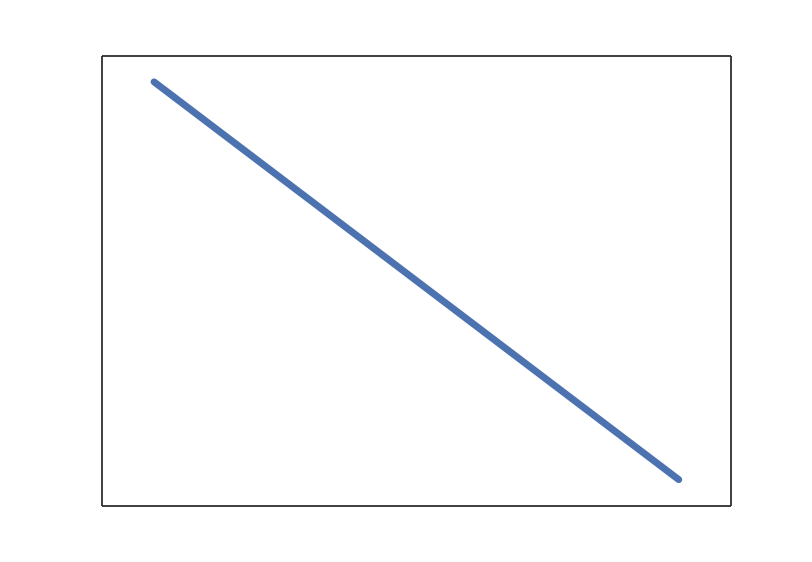
\includegraphics[height=2cm]{figs/kernel/kernelLIN.png} & 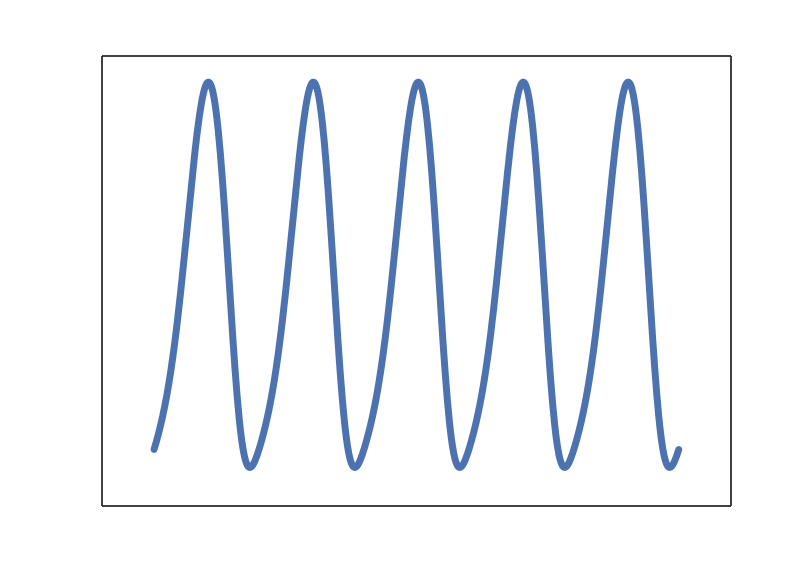
\includegraphics[height=2cm]{figs/kernel/kernelPER.png} & 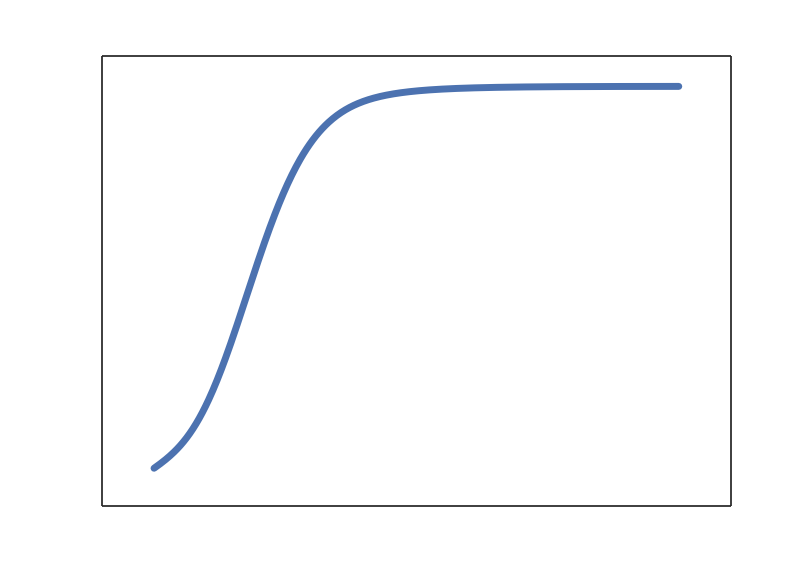
\includegraphics[height=2cm]{figs/kernel/kernelSE.png} & 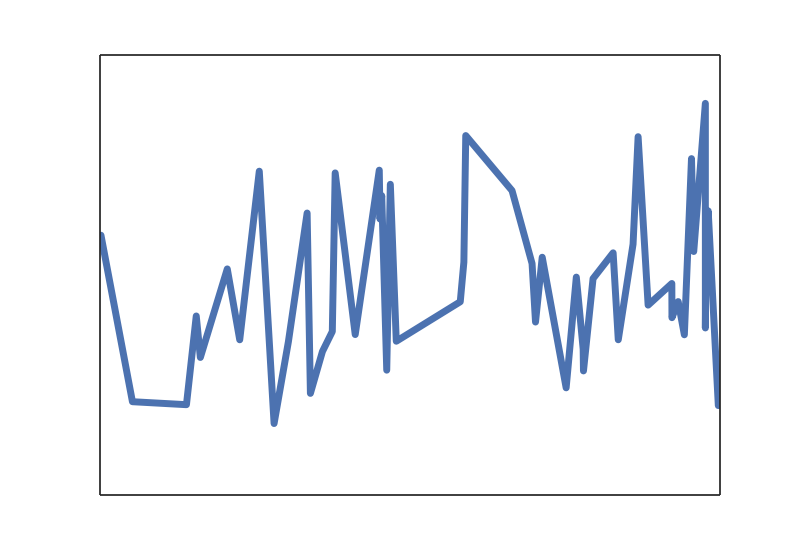
\includegraphics[height=2cm]{figs/kernel/kernelWN.png}\\
\end{tabular}
\begin{tabular}{cccc}
\multicolumn{4}{c}{\bf Composite Structure Examples} \rule{0pt}{0ex}  \\ 
\small LIN + PER: &\small LIN $\times$ PER: &\small SE $\times$ PER: &\small LIN $\times$ LIN: \rule{0pt}{2ex} \\
\small Periodicity with Trend &\small Growing Amplitude &\small Local Periodicity&\small Quadratic \rule{0pt}{2ex} \\
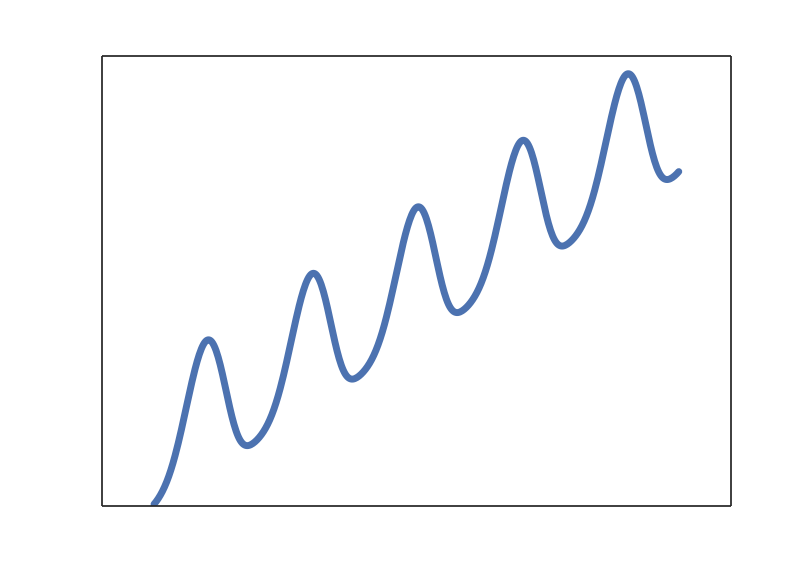
\includegraphics[height=2cm]{figs/kernel/kernelLINplusPER.png} & 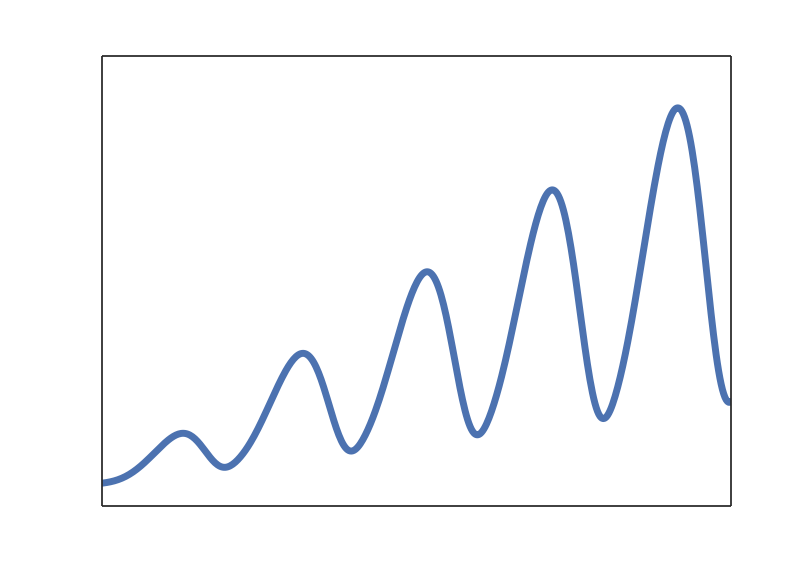
\includegraphics[height=2cm]{figs/kernel/kernelLINtimesPER.png} & 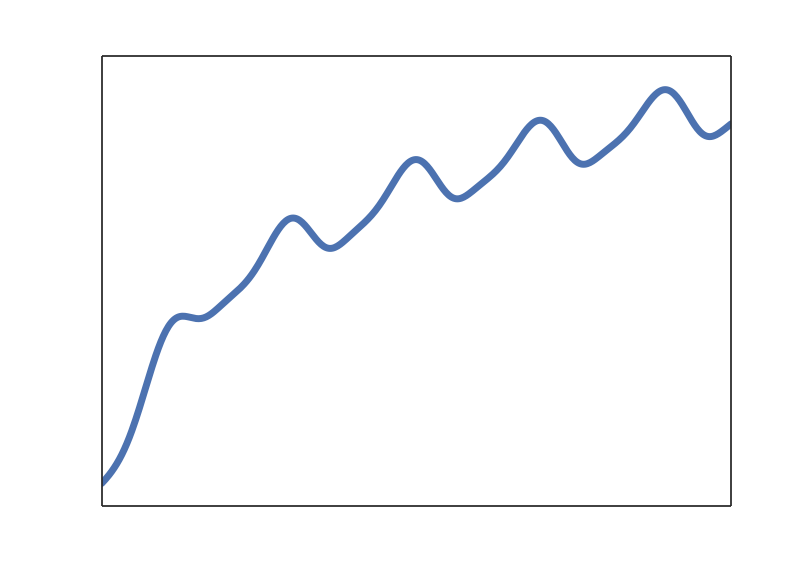
\includegraphics[height=2cm]{figs/kernel/kernelSEplusPER.png}& 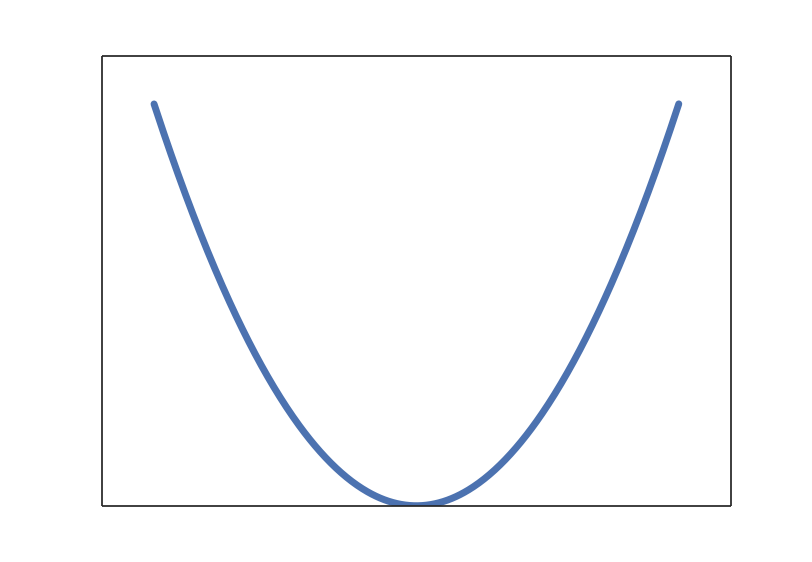
\includegraphics[height=2cm]{figs/kernel/kernelLINtimesLIN.png}\\
\end{tabular}
\caption{}
\end{subfigure}
